\documentclass[10pt,xcolor=dvipsnames]{beamer}
\usepackage[french]{babel}
\usepackage[utf8]{inputenc}
\usepackage[T1]{fontenc}
\usepackage{caption}
\usepackage{algorithm}
\usepackage{algorithmic}
\usepackage{appendixnumberbeamer}
\usepackage{subcaption}
\usetheme[progressbar=frametitle,numbering=fraction]{metropolis}


\setbeamercolor{background canvas}{bg=white}
\setbeamercolor{footline}{fg=gray}
\setbeamertemplate{frame footer}{Rohan Fossé}

\usepackage{booktabs}
\usepackage[scale=2]{ccicons}
\usepackage{tikz}
\usepackage{color}
\usepackage{mathtools}

%% Color Definition

\definecolor{darkspringgreen}{rgb}{0.09, 0.45, 0.27}
\newcommand{\red}[1]{\textcolor{red}{#1}}
\newcommand{\green}[1]{\textcolor{darkspringgreen}{#1}}

\def\checkmark{\tikz\fill[scale=0.4,color=darkspringgreen](0,.35) -- (.25,0) -- (1,.7) -- (.25,.15) -- cycle;}

\long\def\/*#1*/{}

\title{
    Compilation avec Make
}


\subtitle{Slides basées sur celles de Laurent Reveillère}

\date{\centering 2021-2022}
\author{\centering \bf Rohan Fossé}


\begin{document}

\maketitle



  \begin{frame}{Objectifs}
      \begin{itemize}
          \item \textbf{Automatiser} la reconstruction d'un exécutable composé d'un ou plusieurs:
          \begin{itemize}
              \item Modules objets;
              \item Librairies;
              \item Fichier entêtes ...
          \end{itemize}
          \item \textbf{Les avantages}
          \begin{itemize}
              \item Assure la compilation séparée des différentes ressources;
              \item Utilise des macro-commandes et des variables;
              \item Permet de recompiler uniquement le code nécessaire;
              \item Permet d'utiliser des commandes shell arbitraires
              \begin{itemize}
                  \item Scripts d'installation;
                  \item Scripts de désinstallation;
                  \item Scripts de nettoyage...
              \end{itemize}
          \end{itemize}
      \end{itemize}
  \end{frame}

\section{Introduction}

\begin{frame}{Quelques définitions}
\begin{alertblock}{Cible}
    \begin{itemize}
        \item Exécutable à (re)construire;
        \item Commande à exécuter (installation, nettoyage,..).
    \end{itemize}
\end{alertblock}
\begin{alertblock}{Dépendances}
    \begin{itemize}
        \item Élément(s) dont dépend la cible.
    \end{itemize}
\end{alertblock}
\begin{exampleblock}{Exemple en C}
    \begin{itemize}
        \item Cible dépendant d'un fichier \textit{source.c};
        \item Cible construite si le fichier source est plus récent que la cible;
    \end{itemize}
\end{exampleblock}
    \begin{alertblock}{Fichier Makefile}
    Fichier contenant la définition des \alert{dépendances} et des règles de \alert{reconstruction} des cibles.
    \end{alertblock}
\end{frame}


\begin{frame}{Règles de reconstruction d'une cible}
\begin{exampleblock}{Forme générale}
CIBLE(s):DEPENDANCES\\
<tab> COMMANDE(s)
\end{exampleblock}

\begin{exampleblock}{Contraintes syntaxiques}
\begin{itemize}
    \item Cibles et dépendances sont sur une même ligne;
    \item Les commandes commençent \green{\bf{toujours}} par une tabulation;
    \item Commandes sur plusieurs lignes
    \begin{itemize}
        \item Chaque ligne est séparée par le caractère $\diagdown$ sauf la \green{\bf{dernière ligne}}.
        
    \end{itemize}
\end{itemize}
\end{exampleblock}
\end{frame}

\begin{frame}{Exemples}
    \only<1-2>{
        \begin{figure}
            \centering
            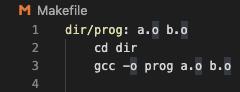
\includegraphics{figures/exemple_1.png}
            \label{fig:my_label}
        \end{figure}
        Est-ce-que cette cible est correctement écrite ? 
        \only<2>{
            \begin{center}
                \red{\Huge $\times$}
            \end{center}
        }
    }
    
    
    \only<3-4>{
        \begin{figure}
            \centering
            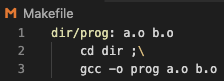
\includegraphics{figures/exemple_2.png}
            \label{fig:my_label}
        \end{figure}
        Est-ce-que cette cible est correctement écrite ? 
        \only<4>{
            \begin{center}
                \green{\Huge \checkmark}
            \end{center}
        }
    }
    
\end{frame}

\begin{frame}{Prenons un vrai exemple}
    \begin{figure}
\centering
    \begin{subfigure}[b]{0.32\textwidth}
        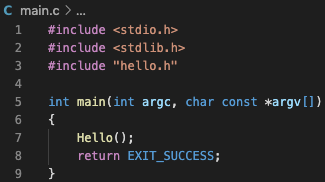
\includegraphics[width=\textwidth]{figures/hello_main.png}
        \label{fig:nature1}
    \end{subfigure}
    \begin{subfigure}[b]{0.32\textwidth}
        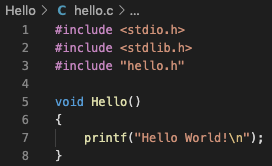
\includegraphics[width=\textwidth]{figures/hello_c.png}
        \label{fig:nature2}
    \end{subfigure}
    \begin{subfigure}[b]{0.32\textwidth}
        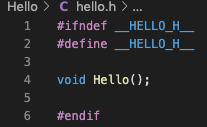
\includegraphics[width=\textwidth]{figures/hello_h.png}
        \label{fig:nature3}
    \end{subfigure}
\caption{Les fichiers considérés pour l'exemple}
\label{fig:images}
\end{figure}
\end{frame}

\begin{frame}{A quoi va ressembler le Makefile ?}
    \begin{figure}
        \centering
        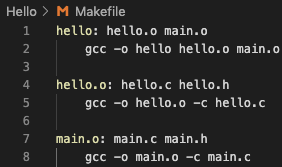
\includegraphics[scale=0.8]{figures/makefile_hello.png}
        \label{fig:my_label}
    \end{figure}
\end{frame}

\begin{frame}{Evaluation d'un fichier Makefile}

\begin{minipage}[t]{0.4\textwidth}
    \begin{figure}
        \centering
        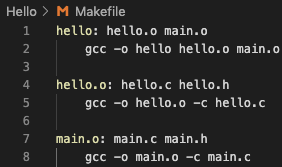
\includegraphics[scale=0.4]{figures/makefile_hello.png}
        \label{fig:my_label}
    \end{figure}
\end{minipage}
\begin{minipage}[t]{0.55\textwidth}
\begin{itemize}
    \item Commande \green{make} sans argument => La première ligne est évaluée;
    \item Commande \green{make} avec argument => Le nom de la règle passée en argument est évaluée;
    \begin{itemize}
        \item exemple: \textit{make hello}
    \end{itemize}
\item Évaluation d'une règle:
\begin{itemize}
    \item Analyse des dépendances
    \item Si une dépendance est la cible d'une autre règle du Makefile, cette règle est à son tour évaluée;
    \item Sinon, les différentes commandes de la règle sont exécutées
\end{itemize}
\end{itemize}
\end{minipage}
\end{frame}

\begin{frame}{Et si je fais un \textit{make} dans notre exemple ?}
    
    \begin{minipage}[t]{0.4\textwidth}
    \begin{figure}
        \centering
        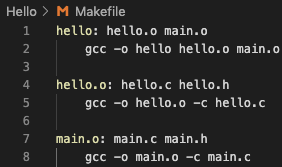
\includegraphics[scale=0.4]{figures/makefile_hello.png}
        \label{fig:my_label}
    \end{figure}
\end{minipage}
\begin{minipage}[t]{0.55\textwidth}
\begin{enumerate}[<+->]
\item La première règle du Makefile est la règle \green{hello}
\item Evaluation de la règle \green{hello}
\item Analyse des dépendances
\begin{enumerate}
    \item Evaluation des cibles \green{hello.o} et \green{main.o}
    \item Analyses des dépendances pour la cible \green{hello.o}
    \item analyses des dépendances pour la cible \green{main.o}
    \item Exécution des commandes si nécessaires
\end{enumerate}
\item Exécution de la commande si nécessaire
\end{enumerate}
\end{minipage}
    
\end{frame}

\begin{frame}{Cibles standard}
\begin{exampleblock}{all}
    Première règle explicite pour définir ce qui est fait par défaut
\end{exampleblock}
    \begin{exampleblock}{install}
    Création de la structure du répertoire, copie des fichiers, ...
    \end{exampleblock}
    \begin{exampleblock}{uninstall}
    Défait ce que \green{install} à fait mais ne supprime pas les fichiers temporaires
    \end{exampleblock}
    \begin{exampleblock}{clean}
    Supprime du répertoire courant tous les fichier temporaires
    \end{exampleblock}
    \begin{exampleblock}{mrproper}
    Remet les répertoires sources dans leur état initial
    \end{exampleblock}
\end{frame}


\begin{frame}{Exemple des cibles standard}
\begin{figure}
    \centering
    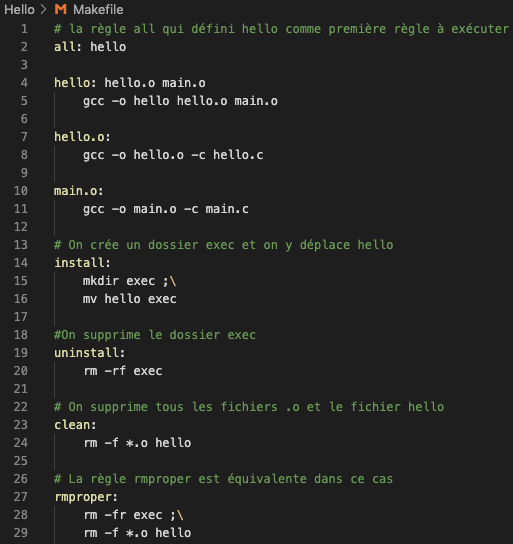
\includegraphics[scale=0.4]{figures/makefile_hello_2.png}
    \label{fig:my_label}
\end{figure}
    
\end{frame}

\begin{frame}{Notion de variables}
    \begin{exampleblock}{Motivations}
    \begin{itemize}
        \item Simplifie l'évolution des règles
        \item Factorise la définition des outils utilisés
    \end{itemize}
    \end{exampleblock}
    \begin{exampleblock}{Définition}
    NOM\_VARIABLE = VALEUR
    \end{exampleblock}
    \begin{exampleblock}{Utilisation}
    $\$(NOM\_VARIABLE)$
    \end{exampleblock}
    \begin{exampleblock}{Exemple}
    \begin{figure}
        \centering
        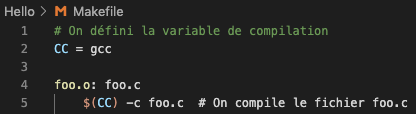
\includegraphics[scale=0.6]{figures/makefile_variable.png}
        \label{fig:my_label}
    \end{figure}
    \end{exampleblock}
\end{frame}

\begin{frame}{Noms de variables standards}
    \begin{exampleblock}{CC}
    Compilateur C
    \end{exampleblock}
    \begin{exampleblock}{RM}
    Commande pour effacer un fichier
    \end{exampleblock}
    \begin{exampleblock}{CFLAGS}
    Paramètres à passer au compilateur C
    \end{exampleblock}
    \begin{exampleblock}{LflAGS}
    Paramètres à passer à l'éditeur de lien
    \end{exampleblock}
    \begin{exampleblock}{EXEC}
    Nom de l'exécutable principal à générer
    \end{exampleblock}
\end{frame}

\begin{frame}{Exemple}
    \begin{figure}
        \centering
        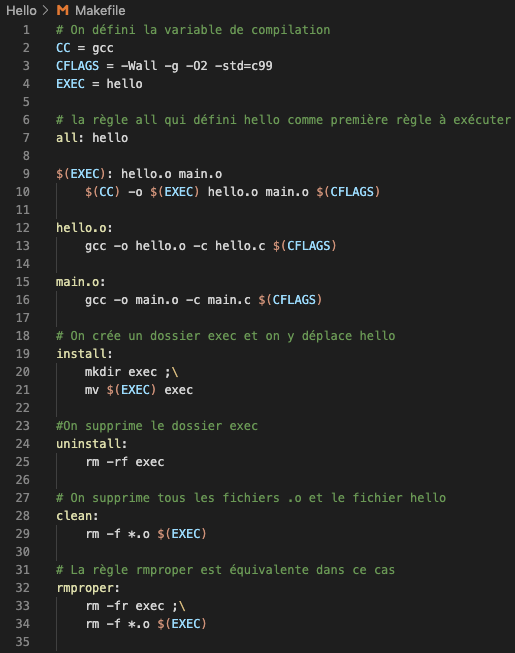
\includegraphics[scale=0.35]{figures/makefile_variable_2.png}
        \label{fig:my_label}
    \end{figure}
\end{frame}

\begin{frame}{Variables automatiques}
    \begin{exampleblock}{\$@}
    Nom de la cible de la règle
    \end{exampleblock}
    \begin{exampleblock}{\$<}
    Nom de la première dépendance
    \end{exampleblock}
    
    \begin{exampleblock}{\$?}
    Nom de toutes les dépendances qui sont plus récentes que la cible
    \end{exampleblock}
\end{frame}

\begin{frame}{Règles implicites}
    \begin{exampleblock}{Objectif}
    \begin{itemize}
        \item Construction d'un module objet (.o) à partir d'un fichier source (.c)
        \item Règles appelées automatiquement pour construire toutes les cibles ayant pour suffixe .o
    \end{itemize}
    \end{exampleblock}
    
    \begin{exampleblock}{Syntaxe}
    \%.o : \%.c\\
    		commandes 
    \end{exampleblock}
\end{frame}




\end{document}

